% ------------------------------------------------------------------------
% ------------------------------------------------------------------------
% abnTeX2: Modelo de Trabalho Academico (tese de doutorado, dissertacao de
% mestrado e trabalhos monograficos em geral) em conformidade com
% ABNT NBR 14724:2011: Informacao e documentacao - Trabalhos academicos -
% Apresentacao
% ------------------------------------------------------------------------
% ------------------------------------------------------------------------
\documentclass[
	% -- opções da classe memoir --
	12pt,				% tamanho da fonte
	openright,			% capítulos começam em pág ímpar (insere página vazia caso preciso)
	oneside,			% para impressão em recto e verso. Oposto a oneside
	a4paper,			% tamanho do papel.
	% -- opções da classe abntex2 --
	% chapter=TITLE,		% títulos de capítulos convertidos em letras maiúsculas
	% section=TITLE,		% títulos de seções convertidos em letras maiúsculas
	% subsection=TITLE,	% títulos de subseções convertidos em letras maiúsculas
	%subsubsection=TITLE,% títulos de subsubseções convertidos em letras maiúsculas
	% -- opções do pacote babel --
	english,			% idioma adicional para hifenização
	brazil,				% o último idioma é o principal do documento
	]{abntex2}

% ---
% Pacotes básicos
% ---
\usepackage{lmodern}			% Usa a fonte Latin Modern
\usepackage[T1]{fontenc}		% Selecao de codigos de fonte.
\usepackage[utf8]{inputenc}		% Codificacao do documento (conversão automática dos acentos)
\usepackage{lastpage}			% Usado pela Ficha catalográfica
\usepackage{indentfirst}		% Indenta o primeiro parágrafo de cada seção.
\usepackage{color}				% Controle das cores
\usepackage{graphicx}			% Inclusão de gráficos
\usepackage{microtype} 			% para melhorias de justificação
% ---

% ---
% Pacotes adicionais, usados apenas no âmbito do Modelo Canônico do abnteX2
% ---
\usepackage{lipsum}				% para geração de dummy text
% ---

% ---
% Pacotes de citações
% ---
\usepackage[brazilian,hyperpageref]{backref}	 % Paginas com as citações na bibl
\usepackage[alf]{abntex2cite}	% Citações padrão ABNT

% ---
% CONFIGURAÇÕES DE PACOTES
% ---

% ---
% Configurações do pacote backref
% Usado sem a opção hyperpageref de backref
\renewcommand{\backrefpagesname}{Citado na(s) página(s):~}
% Texto padrão antes do número das páginas
\renewcommand{\backref}{}
% Define os textos da citação
\renewcommand*{\backrefalt}[4]{
	\ifcase #1 %
		Nenhuma citação no texto.%
	\or
		Citado na página #2.%
	\else
		Citado #1 vezes nas páginas #2.%
	\fi}%
% ---

% ---
% Informações de dados para CAPA e FOLHA DE ROSTO
% ---
\titulo{Desenvolvimento de um sistema de resposta interativo para auxiliar
o ensino-aprendizagem no meio acadêmico}
\autor{Pedro Henrique Araújo Sobral}
\local{Juazeiro, Bahia, Brasil}
\data{2016, v-0.0.1}
\orientador{Max Santana Rolemberg Farias}
\coorientador{João Carlos Sedraz Silva}
\instituicao{%
  \textsc{Universidade Federal do Vale do São Francisco} -- UNIVASF
  \par
  \textsc{Colegiado de Engenharia de Computação}
 % \par
 }
\tipotrabalho{Trabalho de Conclusão de Curso}
% O preambulo deve conter o tipo do trabalho, o objetivo,
% o nome da instituição e a área de concentração
\preambulo{
Trabalho de conclusão de curso \mbox{apresentado} a
Universidade Federal do Vale do São \mbox{Francisco},
Campus Juazeiro, como requisito da obtenção do
título de Engenheiro de \mbox{Computação}.}
% ---


% ---
% Configurações de aparência do PDF final

% alterando o aspecto da cor azul
\definecolor{blue}{RGB}{41,5,195}

% informações do PDF
\makeatletter
\hypersetup{
     	%pagebackref=true,
		pdftitle={\@title},
		pdfauthor={\@author},
    	pdfsubject={\imprimirpreambulo},
	    pdfcreator={LaTeX with abnTeX2},
		pdfkeywords={abnt}{latex}{abntex}{abntex2}{trabalho acadêmico},
		colorlinks=true,       		% false: boxed links; true: colored links
    	linkcolor=blue,          	% color of internal links
    	citecolor=blue,        		% color of links to bibliography
    	filecolor=magenta,      		% color of file links
		urlcolor=blue,
		bookmarksdepth=4
}
\makeatother
% ---

% ---
% Espaçamentos entre linhas e parágrafos
% ---

% O tamanho do parágrafo é dado por:
\setlength{\parindent}{1.3cm}

% Controle do espaçamento entre um parágrafo e outro:
\setlength{\parskip}{0.2cm}  % tente também \onelineskip

% ---
% compila o indice
% ---
% \makeindex
% --


\includeonly{
  pretextual/fichacatalografica,
  pretextual/errata,
  pretextual/folhadeaprovacao,
  pretextual/dedicatoria,
  pretextual/agradecimentos,
  pretextual/epigrafe,
  pretextual/resumo,
  pretextual/listas,
  textual/introducao,
	textual/desenvolvimento,
	textual/materiaisEmetodos,
  textual/referencialteorico,
  textual/produto,
  textual/experimentos,
  textual/consideracoes,
  postextual/anexos,
  postextual/apendice,
  postextual/glosario,
  postextual/indiceremissivo,
}

% ----
% Início do documento
% ----
\begin{document}

% Seleciona o idioma do documento (conforme pacotes do babel)
%\selectlanguage{english}
\selectlanguage{brazil}

% Retira espaço extra obsoleto entre as frases.
\frenchspacing

% ----------------------------------------------------------
% ELEMENTOS PRÉ-TEXTUAIS
% ----------------------------------------------------------
% \pretextual

% ---
% Capa
% ---
\imprimircapa
% ---

% ---
% Folha de rosto
% (o * indica que haverá a ficha bibliográfica)
% ---
\imprimirfolhaderosto*
% ---

% ---
% Inserir a ficha bibliografica
% ---
% % Isto é um exemplo de Ficha Catalográfica, ou ``Dados internacionais de
% catalogação-na-publicação''. Você pode utilizar este modelo como referência.
% Porém, provavelmente a biblioteca da sua universidade lhe fornecerá um PDF
% com a ficha catalográfica definitiva após a defesa do trabalho. Quando estiver
% com o documento, salve-o como PDF no diretório do seu projeto e substitua todo
% o conteúdo de implementação deste arquivo pelo comando abaixo:
%
% \begin{fichacatalografica}
%     \includepdf{fig_ficha_catalografica.pdf}
% \end{fichacatalografica}

\begin{fichacatalografica}
	\sffamily
	\vspace*{\fill}					% Posição vertical
	\begin{center}					% Minipage Centralizado
	\fbox{\begin{minipage}[c][8cm]{13.5cm}		% Largura
	\small
	\imprimirautor
	%Sobrenome, Nome do autor

	\hspace{0.5cm} \imprimirtitulo  / \imprimirautor. --
	\imprimirlocal, \imprimirdata-

	\hspace{0.5cm} \pageref{LastPage} p. : il. (algumas color.) ; 30 cm.\\

	\hspace{0.5cm} \imprimirorientadorRotulo~\imprimirorientador\\

	\hspace{0.5cm}
	\parbox[t]{\textwidth}{\imprimirtipotrabalho~--~\imprimirinstituicao,
	\imprimirdata.}\\

	\hspace{0.5cm}
		1. Palavra-chave1.
		2. Palavra-chave2.
		2. Palavra-chave3.
		I. Orientador.
		II. Universidade xxx.
		III. Faculdade de xxx.
		IV. Título
	\end{minipage}}
	\end{center}
\end{fichacatalografica}
% --


% ---
% Inserir errata
% ---
% \begin{errata}
Elemento opcional da \citeonline[4.2.1.2]{NBR14724:2011}. Exemplo:

\vspace{\onelineskip}

FERRIGNO, C. R. A. \textbf{Tratamento de neoplasias ósseas apendiculares com
reimplantação de enxerto ósseo autólogo autoclavado associado ao plasma
rico em plaquetas}: estudo crítico na cirurgia de preservação de membro em
cães. 2011. 128 f. Tese (Livre-Docência) - Faculdade de Medicina Veterinária e
Zootecnia, Universidade de São Paulo, São Paulo, 2011.

\begin{table}[htb]
\center
\footnotesize
\begin{tabular}{|p{1.4cm}|p{1cm}|p{3cm}|p{3cm}|}
  \hline
   \textbf{Folha} & \textbf{Linha}  & \textbf{Onde se lê}  & \textbf{Leia-se}  \\
    \hline
    1 & 10 & auto-conclavo & autoconclavo\\
   \hline
\end{tabular}
\end{table}

\end{errata}
% ---


% ---
% Inserir folha de aprovação
% ---
% % Isto é um exemplo de Folha de aprovação, elemento obrigatório da NBR
% 14724/2011 (seção 4.2.1.3). Você pode utilizar este modelo até a aprovação
% do trabalho. Após isso, substitua todo o conteúdo deste arquivo por uma
% imagem da página assinada pela banca com o comando abaixo:
%
% \includepdf{folhadeaprovacao_final.pdf}
%
\begin{folhadeaprovacao}

  \begin{center}
    {\ABNTEXchapterfont\large\imprimirautor}

    \vspace*{\fill}\vspace*{\fill}
    \begin{center}
      \ABNTEXchapterfont\bfseries\Large\imprimirtitulo
    \end{center}
    \vspace*{\fill}

    \hspace{.45\textwidth}
    \begin{minipage}{.5\textwidth}
        \imprimirpreambulo
    \end{minipage}%
    \vspace*{\fill}
   \end{center}

   Trabalho aprovado. \imprimirlocal, 25 de Agosto de 2016:

   \assinatura{\textbf{\footnotesize{Orientador (\textsc{CCOMP/UNIVASF)}}}\\ \imprimirorientador}
   \assinatura{\textbf{\footnotesize{Professor (CCOMP/UNIVASF)}} \\ Dr. Brauliro Gonçalves Leal}
   \assinatura{\textbf{\footnotesize{Professor (CCIVIL/UNIVASF)}} \\ Me. João Carlos Sedraz Silva}

   \begin{center}
    \vspace*{0.5cm}
    {\large\imprimirlocal}
    \par
    {\large\imprimirdata}
    \vspace*{1cm}
  \end{center}

\end{folhadeaprovacao}
% ---


% ---
% Dedicatória
% ---
% \begin{dedicatoria}
   \vspace*{\fill}
   \centering
   \noindent
   \textit{ Este trabalho é dedicado às crianças adultas que,\\
   quando pequenas, sonharam em se tornar cientistas.} \vspace*{\fill}
\end{dedicatoria}
% ---


% ---
% Agradecimentos
% ---
% \begin{agradecimentos}

PRIMEIRO DE TUDO SO QUERO AGRADECER A GOD!
PRIMEIRO DE TUDO SO QUERO AGRADECER A GOD!
PRIMEIRO DE TUDO SO QUERO AGRADECER A GOD!
PRIMEIRO DE TUDO SO QUERO AGRADECER A GOD!

Os agradecimentos principais são direcionados à Gerald Weber, Miguel Frasson,
Leslie H. Watter, Bruno Parente Lima, Flávio de Vasconcellos Corrêa, Otavio Real
Salvador, Renato Machnievscz\footnote{Os nomes dos integrantes do primeiro
projeto abn\TeX\ foram extraídos de
\url{http://codigolivre.org.br/projects/abntex/}} e todos aqueles que
contribuíram para que a produção de trabalhos acadêmicos conforme
as normas ABNT com \LaTeX\ fosse possível.

Agradecimentos especiais são direcionados ao Centro de Pesquisa em Arquitetura
da Informação\footnote{\url{http://www.cpai.unb.br/}} da Universidade de
Brasília (CPAI), ao grupo de usuários
\emph{latex-br}\footnote{\url{http://groups.google.com/group/latex-br}} e aos
novos voluntários do grupo
\emph{\abnTeX}\footnote{\url{http://groups.google.com/group/abntex2} e
\url{http://www.abntex.net.br/}}~que contribuíram e que ainda
contribuirão para a evolução do \abnTeX.

\end{agradecimentos}
% ---


% ---
% Epígrafe
% ---
% \begin{epigrafe}
    \vspace*{\fill}
	\begin{flushright}
    \textit{
    ``Diga-me eu esquecerei,\\
        ensina-me e eu poderei lembrar,\\
        envolva-me e eu aprenderei.''\\
        (Benjamin Franklin)}
	\end{flushright}
\end{epigrafe}
% ---


% ---
% RESUMOS
% ---
% % resumo em português
\setlength{\absparsep}{18pt} % ajusta o espaçamento dos parágrafos do resumo
\begin{resumo}
  Sistemas de resposta em sala de aula permitem ao professor um retorno
  em tempo real sobre o entendimento de toda uma classe sobre um determinado
  tópico de estudo. Essa informação é valiosa porque permite ao educador, por exemplo,
  realizar uma avaliação formativa, orientando-o na prática pedagógica.
  No entanto, o custo associado à aquisição dos sistemas de resposta podem ser proibitivos ao uso.
  É importante destacar essa tecnologia apenas como um meio para colaborar no processo
  de ensino e aprendizagem, e só faz sentido quando associada com práticas
  pedagógicas de ensino como o aprendizado ativo.
  Dessa forma, nesse trabalho foi desenvolvido um sistema de resposta em sala de aula,
  que possibilite aos professores e aos estudantes uma ferramenta de software livre, que permita
  usar \textit{smartphones} como sistema de resposta.

 \textbf{Palavras-chave}:  Aprendizado Ativo. Instrução pelos Colegas. Sistemas de Resposta em Sala de Aula. Aplicativos Híbridos para Celular.
\end{resumo}

% resumo em inglês
\begin{resumo}[Abstract]
 \begin{otherlanguage*}{english}
   Classroom response systems (CRS) or just clickers allow the teacher a real-time feedback on the understanding of a whole class on a topic of study. This information is valuable because it allows the educator, for example, conduct a formative assessment, guiding it in pedagogical practice.
   However, it is important to highlight this technology only as a means to assist in the process of teaching and learning, and only makes sense when combined with pedagogical practices of teaching and active learning. Moreover, the cost associated with clickers can be prohibitive to use. Thus, this work will develop a CRS that allows teachers and students a free software that will give them the opportunity to use smartphones as clickers so that it can be mainly used for educational practices of active learning as Peer Instruction.

   \noindent
   \textbf{Keywords}: Active Learning. Peer Instruction. Classroom Response Systems. Hybrid Mobile Applications.
 \end{otherlanguage*}
\end{resumo}


% ---
% LISTAS
% ---
% % ---
% inserir lista de ilustrações
% ---
% \pdfbookmark[0]{\listfigurename}{lof}
% \listoffigures*
% \cleardoublepage
% ---

% ---
% inserir lista de tabelas
% ---
% \pdfbookmark[0]{\listtablename}{lot}
% \listoftables*
% \cleardoublepage
% ---

% ---
% inserir lista de abreviaturas e siglas
% ---
% \begin{siglas}
%  \item[ABNT] Associação Brasileira de Normas Técnicas
%  \item[abnTeX] ABsurdas Normas para TeX
% \end{siglas}

% \renewcommand{\nomname}{Lista de abreviaturas e siglas}
% \printnomenclature
% \cleardoublepage

% ---

% ---
% inserir lista de símbolos
% ---
% \begin{simbolos}
%  \item[$ \Gamma $] Letra grega Gama
%  \item[$ \Lambda $] Lambda
%  \item[$ \zeta $] Letra grega minúscula zeta
%  \item[$ \in $] Pertence
% \end{simbolos}
% ---

% ---
% inserir o sumario
% ---
\pdfbookmark[0]{\contentsname}{toc}
\tableofcontents*
\cleardoublepage
% ---



% ----------------------------------------------------------
% ELEMENTOS TEXTUAIS
% ----------------------------------------------------------
\textual
% ---
\chapter{Introdução}

Assim como o artista propõe a sua obra ao público, assim deve ser o professor que
propõe conhecimento aos seus estudantes. No entanto, hoje parece que ainda prevalece
o modelo em que o professor é o transmissor de informações em aulas puramente expositivas,
em que prevalece a baixa participação dos alunos \cite[p. 8]{Silva2001}.

Por que ainda se justifica o modelo de ensino em que se baseia
na disseminação de informações, que nunca foi tão fácil achar (internet,
livros, etc)? O ensino de hoje deveria estar focado para uma nova
visão em que o papel do professor seja de intermediar o ensino \cite[p. 19]{Araujo2013}.

Sistemas de respostas são sistemas que possibilitam que todos os alunos
respondam a questões apresentadas no projetor. Geralmente um gráfico de barras
é apresentado logo em seguida que os estudantes submetem as suas soluções
utilizando algum dispositivo remoto. As respostas são anônimas para os seus colegas,
no entanto o professor pode identificar cada estudante individualmente pela
identificação única do dispositivo, permitindo assim uma análise individual \cite[p. 1]{Kay2009}.


Esse resultado imediato pode ser usado juntamente
com metodos que promovem a interação social voltada para a aprendizagem como a
Instrução pelos Colegas (IpC) que tem alcançado sucesso internacionalmente \cite[p. 3]{Araujo2013}.

\section{Objetivo Geral}
Desenvolver um sistema de resposta em sala de aula,
que possibilite aos professores e aos estudantes uma ferramenta de software livre,
que permita usar {\textit{smartphones}} como {\clickers} para que o mesmo possa
ser usado principalmente com práticas pedagógicas de aprendizado ativo como o IpC.

\section{Objetivos Específicos}

\begin{itemize}
    \item Realizar levantamento de requisitos sobre os sistemas de resposta em sala de aula;
    \item Especificar e implementar uma aplicação para dispositivos móveis, que será utilizado como {\clickers};
    \item Especificar e implementar uma aplicação web para o professor administrar as questões e gerar relatórios;
    \item Especificar e implementar um sistema servidor, para receber e
    enviar dados para os os clientes: dispositivos móveis dos alunos e navegador
    web do professor.
\end{itemize}

\section{Organização do texto}
Além desta introdução, este trabalho está dividido em mais dois capítulos.

\begin{description}
  \item[Revisão de literatura:] Esse capítulo discute um contexto pedagógico
  para o uso de sistemas de resposta em sala de aula. Inicialmente, é
  apresentado o conceito de aprendizado ativo e um método de implementação: Instrução pelos Colegas.
  Em seguida, são apontados os sistemas de resposta em sala de aula como uma
  ferramenta para ajudar o professor a mediar um aprendizado significativo  em
  sala de aula. O capítulo é encerrado apresentando os benefícios e desafios de uso dessa tecnologia.

  \item[Material e Métodos:] Nesse capítulo serão descritas as fases de especificação e projeto do sistema.
  Ainda nesse capítulo são apresentadas as ferramentas e a arquitetura
  do sistema, dando uma visão geral do que foi desenvolvido.

\end{description}

\chapter{Referencial Teórico}

\section{Aprendizado Ativo}
Método pedagógico que envolve os estudantes no aprendizado, de maneira bastante simples
essa é a definição de aprendizado ativo. Em resumo, aprendizado ativo é qualquer coisa
que além de envolver os estudantes no fazer, os faça pensar no que estão fazendo \cite[p. 19]{Charles1991}.
Os princípios do aprendizado ativo são dois: envolver os estudantes em atividades
(discutir, ler, escrever, resolver) e promover o envolvimento dos alunos  \cite[p. 3]{Prince2004}.

{\color{red}TALVEZ FALAR SOBRE APRENDIZAGEM PASSIVA (BANCARIA) DE PAULO FREIRE!}

Em salas de aula que utilizam o aprendizado ativo pode-se ter um aumento de até 6\%
na média final nas provas dos alunos e que aquelas salas de aula puramente expositivas
têm 55\% mais chance de reprovarem os alunos do que aquelas com aprendizado ativo.
Esse aumento que pode parecer pouco (0,3 no GPA) colocaria a média daqueles estudantes
que desistem do curso bem próximo daqueles que permanecem, podendo-se então aumentar
a taxa de retenção dos estudantes \cite[p. 4]{Freeman2014}.

O estudo de meta-análise de \citeonline{Freeman2014} envolveu mais de 200 artigos
que comparavam as performances dos alunos em salas de aula com pelo menos algum
elemento de aprendizado ativo com as tradicionais aulas expositivas. Além de
mostrarem evidências de que o aprendizado ativo pode melhorar o aprendizado dos
estudantes de graduação principalmente nas áreas de ciência, tecnologia, engenharia
e matemática, \citeauthoronline{Freeman2014} propõem aos futuros pesquisadores
testarem não mais a eficiência dos métodos de aprendizado ativo frente as tradicionais
aulas expositivas (``primeira geração de pesquisas''), mas sim de verificar qual
o tipo de aprendizado ativo é mais apropriado para cada área do conhecimento
(``segunda geração de pesquisas'').

Tornar o aluno um agente ativo no processo de ensino-aprendizagem dado a realidade brasileira
não é uma tarefa fácil. Muitas são as adversidades de infraestrutura e institucionais
encontradas de modo a propiciar uma aprendizagem significativa. Seja por salas com
numero excessivo de alunos, estes desinteressados, professores mal pagos, ou com
a pressão de produzir cientificamente \cite{Araujo2013}.

No entanto, muitas são as iniciativas encontradas na literatura mostrando resultados
satisfatórios que podem ajudar o professor nesse processo \cite{Crouch2001, Gok2013, Barros2004}.
Na próxima seção será apresentado o método ativo de ensino \textit{Peer Instruction} ou \textit{Instrução pelos Colegas}
(IpC)\nomenclature{IpC}{Instrução pelos Colegas}.

\subsection{Instrução pelos Colegas (IpC)}

O IpC foi desenvolvido pelo Professor Eriz Mazur da Universidade de Harvard (EUA) na
década de 90. O objetivo do IpC é fazer com que todos os estudantes se engajem em
discussões com o vizinho de opinião diferente sobre um determinado conceito e então cada
estudante tenta explicar o conceito um para o outro \cite{Mazur2009}.

No método IpC geralmente o professor começa fazendo uma breve exposição dialogada do conteúdo (15min).
Logo em seguida é colocado para os estudantes uma questão conceitual, que é
desenvolvida de modo a avaliar o entendimento dos estudantes sobre um tópico. Um
exemplo de uma questão conceitual de introdução a física é mostrada na \autoref{fig:desenv_ct}. Os
estudantes então individualmente respondem a questão (1-2min) geralmente utilizando
\textit{clickers} (Ver \autoref{section:sistemas_de_resposta}). Dependendo do percentual de alunos que acertem a questão,
o professor pode revisar o assunto (acerto < 30\%), fazer uma breve explanação da
questão e ir para um próximo tópico ou nova questão (acerto > 70\%), ou o que se
deseja do método, um percentual de acerto entre 30\% e 70\% em que nessa situação o
professor estimula que os alunos encontrem um parceiro que respondeu preferencialmente de forma diferente
e que tentem explicar um para o outro o porquê de estar correto, ou seja, os alunos se auto
instruem temos então o nome do método ``Instrução pelos Colegas'' \cite{Mazur2009, Crouch2001}.
A \autoref{fig:desen_fluxograma_ipc} resume o processo de implementação do método IpC na sala de aula.

\begin{figure}[!htb]
  \centering
  \caption{Exemplo de uma questão conceitual}
  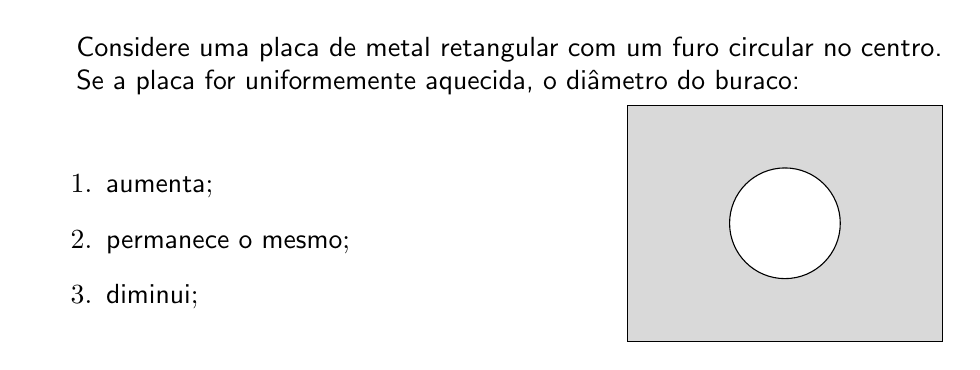
\begin{tikzpicture}[scale=1]
    \label{fig:desenv_ct}
    \node[,text width=11cm] at (0,4) {\textsf{Considere uma placa de metal retangular com um furo circular no centro. Se a
    placa for uniformemente aquecida, o diâmetro do buraco:}};
    \node[,text width=5cm] at (-3.5,2) {
      \begin{enumerate}
        \item \textsf{aumenta};
        \item \textsf{permanece o mesmo};
        \item \textsf{diminui};
      \end{enumerate}
    };
    \draw[fill=gray!30, shift={(1.5cm,.5cm)}](0,0) rectangle (4,3);
    \draw[fill=white, shift={(1.5cm,.5cm)}](2,1.5) circle(20pt);
  \end{tikzpicture}
  \fonte{Adaptado de \cite{Watkins2013}}
\end{figure}

No entanto, a implementação do IpC não ocorre apenas na sala de aula. Espera-se
que os alunos façam leituras e atividades antes da aula. Também espera-se do
professor guiar os estudantes nessa etapa, seja indicando ou disponibilizando o
material adequado. O tempo em sala de aula que seria utilizado para apenas transferir
informações para os estudante é utilizado principalmente para discussões, interação
entre os estudantes, tempo para assimilação e para pensar  \cite{Mazur2009, Crouch2001}.



Lorem ipsum dolor sit amet, consectetur adipisicing elit, sed do eiusmod tempor incididunt ut labore et dolore magna aliqua. Ut enim ad minim veniam, quis nostrud exercitation ullamco laboris nisi ut aliquip ex ea commodo consequat. Duis aute irure dolor in reprehenderit in voluptate velit esse cillum dolore eu fugiat nulla pariatur. Excepteur sint occaecat cupidatat non proident, sunt in culpa qui officia deserunt mollit anim id est laborum.

\begin{figure}[htbp]
  \centering
  \caption{Diagrama do processo de implementação do método IpC}
  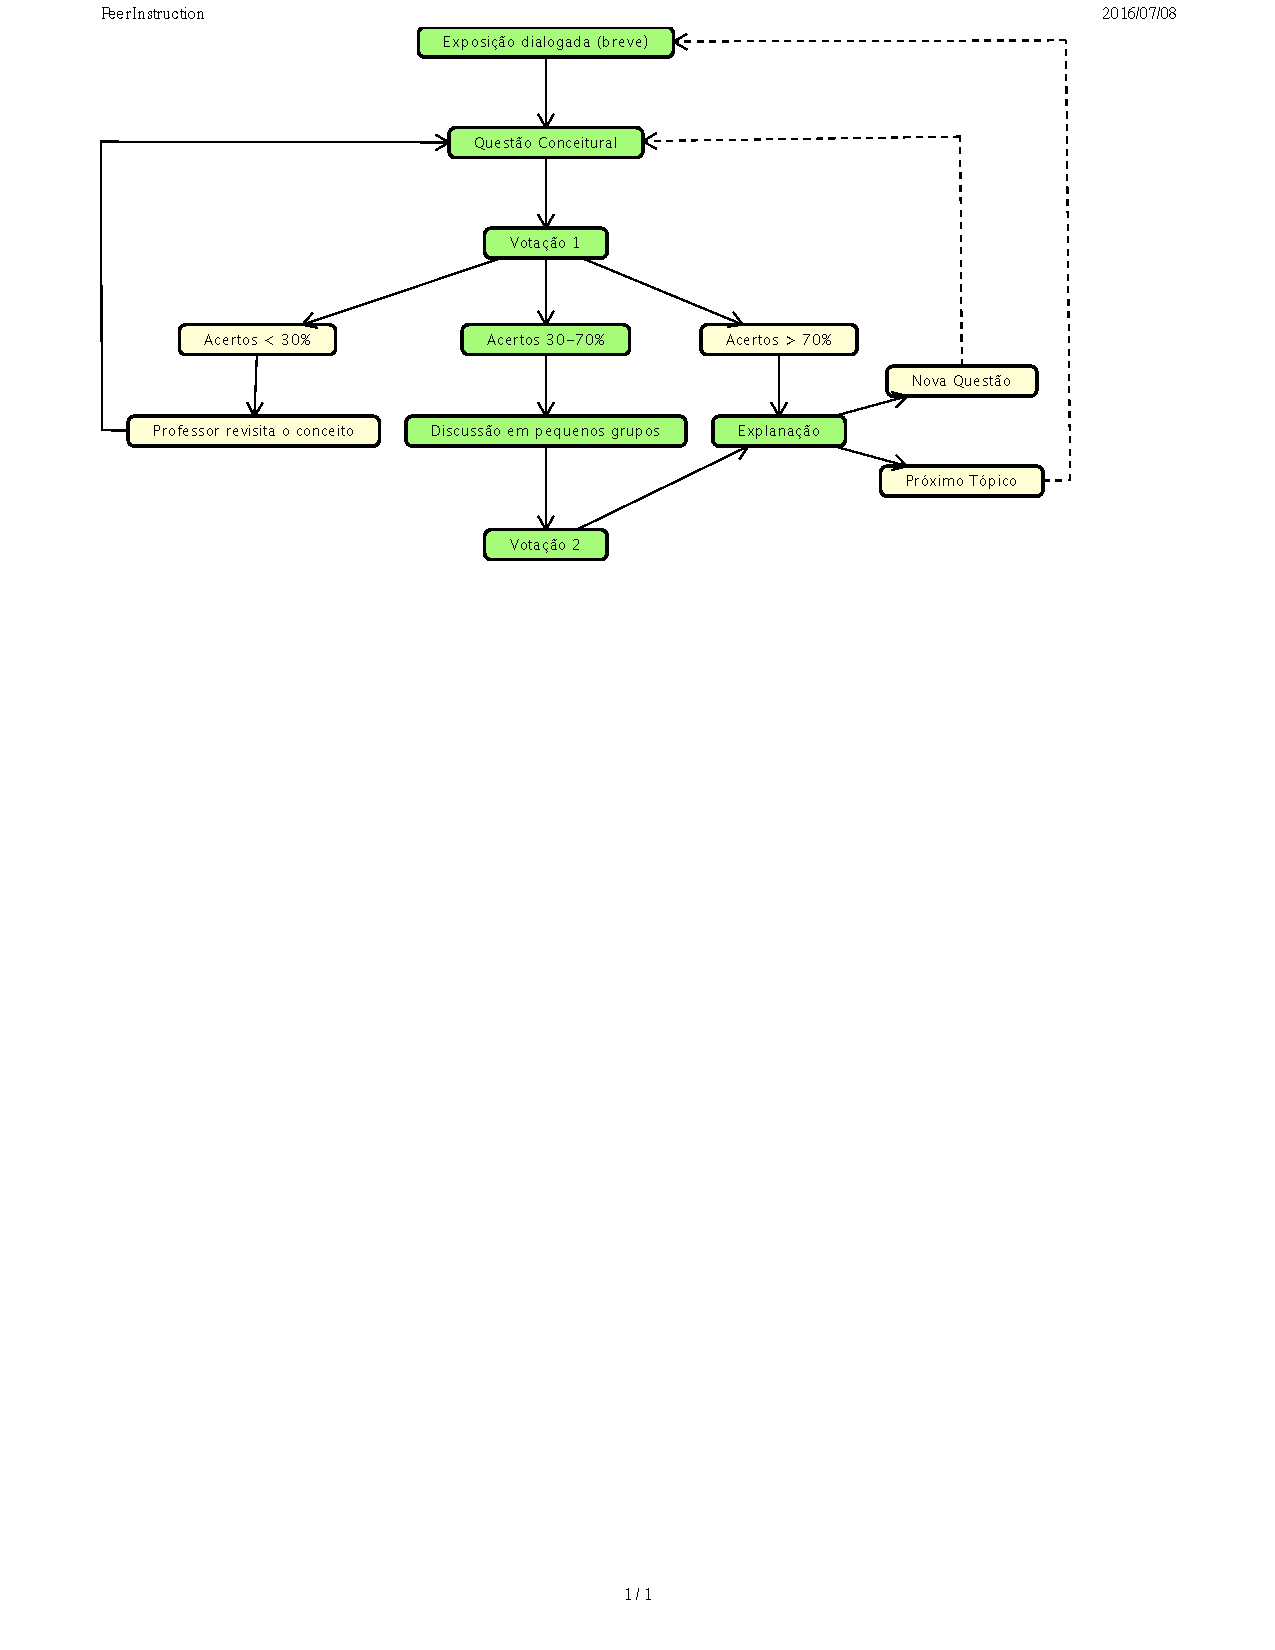
\includegraphics[clip, trim=0cm 18cm 3cm .4cm,scale=0.75]{imagens/peer_instruction}
  \label{fig:desen_fluxograma_ipc}
  \fonte{\cite{X} (Adaptado)}
\end{figure}


\section{Sistemas de Resposta}
\label{section:sistemas_de_resposta}

Com efeito, a tecnologia apresenta-se como meio, como instrumento para colaborar no desenvolvimento do processo de aprendizagem. A tecnologia reveste-se de um valor relativo e dependente desse processo. Ela tem sua importância apenas como um instrumento significativo para favorecer a aprendizagem de alguém. Não é a tecnologia que vai resolver ou solucionar o problema educacional do Brasil. Poderá colaborar, no entanto, se for usada adequadamente, para o desenvolvimento educacional de nossos estudantes.

\chapter{Material e Métodos}



% ----------------------------------------------------------
% ELEMENTOS PÓS-TEXTUAIS
% ----------------------------------------------------------
\postextual
% ----------------------------------------------------------
% Referências bibliográficas
% ----------------------------------------------------------
\bibliography{postextual/referencias}

% ----------------------------------------------------------
% Glossário
% ----------------------------------------------------------
%
% Consulte o manual da classe abntex2 para orientações sobre o glossário.
%
%\glossary


% ----------------------------------------------------------
% Apêndices
% ----------------------------------------------------------
% ---
% Inicia os apêndices
% ---
\begin{apendicesenv}

% Imprime uma página indicando o início dos apêndices
\partapendices

% ----------------------------------------------------------
\chapter{Quisque libero justo}

% ----------------------------------------------------------

\lipsum[50]

% ----------------------------------------------------------
\chapter{Nullam elementum urna vel imperdiet sodales elit ipsum pharetra ligula
ac pretium ante justo a nulla curabitur tristique arcu eu metus}
% ----------------------------------------------------------
\lipsum[55-57]

\end{apendicesenv}
% ---


% ----------------------------------------------------------
% Anexos
% ----------------------------------------------------------
% ---
% Inicia os anexos
% ---
\begin{anexosenv}

% Imprime uma página indicando o início dos anexos
\partanexos

% ---
\chapter{Morbi ultrices rutrum lorem.}
% ---
\lipsum[30]

% ---
\chapter{Cras non urna sed feugiat cum sociis natoque penatibus et magnis dis
parturient montes nascetur ridiculus mus}
% ---

\lipsum[31]

% ---
\chapter{Fusce facilisis lacinia dui}
% ---

\lipsum[32]

\end{anexosenv}


%---------------------------------------------------------------------
% INDICE REMISSIVO
%---------------------------------------------------------------------
% % \phantompart
% \printindex
%---------------------------------------------------------------------



\end{document}
